\documentclass[10pt,t,presentation,ignorenonframetext,aspectratio=169]{beamer}
% \documentclass[10pt,t,handout,ignorenonframetext,aspectratio=169]{beamer}
\usepackage[default]{lato}
\usepackage{tk_beamer1}
\input{tk_packages}
\input{tk_macros}
\input{tk_environ}
\input{tk_ximera}
\usepackage{wasysym}            % for smiley

%%%% META DATA
\newcommand{\semester}{Autumn 2021}
\newcommand{\course}{Math 1151}
\newcommand{\lecTitle}{Lecture 1: Review of Precalculus}

%%%% TITLE PAGE
\title[\course]{\lecTitle}
\institute[Ohio State]
{
  \medskip
}
\date[\week]{\semester}
\author{Tae Eun Kim, Ph.D.}

\begin{document}
\begin{frame}
  \titlepage
\end{frame}

\begin{frame}
  \frametitle{Overview}
  \tableofcontents
\end{frame}

\section{Understanding Functions (UF)}
\label{sec:underst-funct-uf}
\begin{frame}
  \frametitle{``For each input, exactly on output''}
  \begin{definition}\index{function}
    \begin{itemize}
    \item \dfn{function}: a relation between sets where for each
      input, there is exactly one output
    \item \dfn{domain}: the set of the inputs of a function
    \item \dfn{range}: the set of the outputs of a function
    \end{itemize}
  \end{definition}
\end{frame}

\begin{frame}
  \frametitle{Representation of functions}
  \begin{itemize}
  \item \textbf{formula}: $f(x) = x^3$
  \item \textbf{table}: \\
    \begin{center}
      \begin{tabular}{c|c|c|c|c}
        input & 1 & -2 & 1.5 & $\cdots$ \\ \hline
        output & 1 & -8 & 3.375 & $\cdots$
      \end{tabular}
    \end{center}
  \item \textbf{graph}: \\
    \begin{center}
      \begin{tikzpicture}
        \begin{axis}[
          domain=-2:2,
          width=0.6*4in,
          height=0.6*3in,
          axis lines =middle, xlabel=$x$, ylabel=$y$,
          every axis y label/.style={at=(current axis.above origin),anchor=south},
          every axis x label/.style={at=(current axis.right of origin),anchor=west},
          ]
          \addplot [thick, penColor, smooth] {x^3};
        \end{axis}
      \end{tikzpicture}
    \end{center}
  \end{itemize}
\end{frame}

\begin{frame}
  \vs
  \begin{block}{Example: Greatest Integer Function}
    \begin{itemize}
    \item maps any real number $x$ to the greatest integer less than
      or equal to $x$.
    \item a.k.a. \textit{floor function}
    \item denoted by $\lfloor x \rfloor$
    \item many inputs to one output
    \end{itemize}
  \end{block}

  \vfill
  \begin{center}
    \begin{tikzpicture}
      \begin{axis}[
        domain=-2:4,
        width=0.6*4in,
        height=0.6*3in,
        axis lines =middle, xlabel=$x$, ylabel=$y$,
        every axis y label/.style={at=(current axis.above origin),anchor=south},
        every axis x label/.style={at=(current axis.right of origin),anchor=west},
        clip=false,
        % axis on top,
        ]
        \addplot [textColor, very thin, domain=(0:2.3)] {0}; % puts the axis back, axis on top clobbers our open holes
        \addplot [textColor, very thin] plot coordinates {(0,0) (0,2)}; % puts the axis back, axis on top clobbers our open holes
        \addplot [very thick, penColor, domain=(-2:-1)] {-2};
        \addplot [very thick, penColor, domain=(-1:0)] {-1};
        \addplot [very thick, penColor, domain=(0:1)] {0};
        \addplot [very thick, penColor, domain=(1:2)] {1};
        \addplot [very thick, penColor, domain=(2:3)] {2};
        \addplot [very thick, penColor, domain=(3:4)] {3};
        \addplot[color=penColor,fill=penColor,only marks,mark=*] coordinates{(-2,-2)};  %% closed hole
        \addplot[color=penColor,fill=penColor,only marks,mark=*] coordinates{(-1,-1)};  %% closed hole
        \addplot[color=penColor,fill=penColor,only marks,mark=*] coordinates{(0,0)};  %% closed hole
        \addplot[color=penColor,fill=penColor,only marks,mark=*] coordinates{(1,1)};  %% closed hole
        \addplot[color=penColor,fill=penColor,only marks,mark=*] coordinates{(2,2)};  %% closed hole
        \addplot[color=penColor,fill=penColor,only marks,mark=*] coordinates{(3,3)};  %% closed hole
        \addplot[color=penColor,fill=background,only marks,mark=*] coordinates{(-1,-2)};  %% open hole
        \addplot[color=penColor,fill=background,only marks,mark=*] coordinates{(0,-1)};  %% open hole
        \addplot[color=penColor,fill=background,only marks,mark=*] coordinates{(1,0)};  %% open hole
        \addplot[color=penColor,fill=background,only marks,mark=*] coordinates{(2,1)};  %% open hole
        \addplot[color=penColor,fill=background,only marks,mark=*] coordinates{(3,2)};  %% open hole
        \addplot[color=penColor,fill=background,only marks,mark=*] coordinates{(4,3)};  %% open hole
      \end{axis}
    \end{tikzpicture}
    %% \caption{A plot of $f(x)=\lfloor x\rfloor$. Here we can see that for each input (a
    %% value on the $x$-axis), there is exactly one output (a value on the
    %% $y$-axis).}
    %% \label{plot:greatest-integer fxn}
  \end{center}
\end{frame}

\begin{frame}
  \vs
  \begin{theorem}[Vertical line test]
    The curve $y=f(x)$ represents $y$ as a function of $x$ at $x=a$ if and
    only if the vertical line $x=a$ intersects the curve $y=f(x)$ at
    exactly one point. This is called the \dfn{vertical line test}.
  \end{theorem}
\end{frame}

\begin{frame}
  \vs
  \begin{block}{Distinguishing two functions}
    \begin{itemize}
    \item Do they have the same domain?
    \item Do they display the same relation?
    \end{itemize}
  \end{block}

  \vs
  \textbf{Question.} Determine if the two function are the same.
  \begin{enumerate}
  \item $f(x) = \sqrt{x^2}$ and  $g(x) = \abs{x}$ \vfill
  \item $\ds f(x) = \frac{x^2-3x+2}{x-2}$ and $g(x) = x-1$ \vfill
  \end{enumerate}
\end{frame}

\begin{frame}
  \frametitle{Composition of functions}
  \begin{block}{Composite functions}
    \begin{itemize}
    \item can be thought of as putting one function inside another
    \item \textbf{Notation:} $( f \circ g) (x) = f(g(x))$
    \item \textbf{Warning:} The range of inner function must be
      contained in the domain of outer function.
    \end{itemize}
  \end{block}
\end{frame}

\begin{frame}
  \vs
  \textbf{Question.} Study the composition $f \circ g$ where
  \begin{align*}
    f(x)&=x^2 &&\text{for $-\infty< x< \infty$,}\\
    g(x)&= \sqrt{x} &&\text{for $0\le x< \infty$.}
  \end{align*}
  \vfill
\end{frame}

\begin{frame}
  \vs
  \textbf{Question.} Study the composition $f \circ g$.
  \begin{align*}
    f(x)&=\sqrt{x} &&\text{for $0\le x< \infty$,}\\
    g(x)&= x^2 &&\text{for $-\infty< x< \infty$.}
  \end{align*}
  \vfill
\end{frame}

\begin{frame}
  \frametitle{Inverses of functions}
  \begin{definition}
    Let $f$ be a function with domain $A$ and range $B$:
    \[
      f : A \to B
    \]
    % \begin{image}
    %   \begin{tikzpicture}
    %     \node[star,star points=7,star point ratio=2.5,draw] at (0,0) {$A$};
    %     \node[cloud, draw,cloud puffs=10,cloud puff arc=120, aspect=2, inner ysep=1em] at (5,0) {$B$};
    %     \node at (2.25,.3) {$f$};
    %     \draw[->] (1.5,0) to (3,0);
    %   \end{tikzpicture}
    % \end{image}
    Let $g$ be a function with domain $B$ and range $A$:
    \[
      g : B \to A
    \]
    % \begin{image}
    %   \begin{tikzpicture}
    %     \node[cloud, draw,cloud puffs=10,cloud puff arc=120, aspect=2, inner ysep=1em] at (-.5,0) {$B$};
    %     \node[star,star points=7,star point ratio=2.5,draw] at (4.5,0) {$A$};
    %     \node at (2.25,.3) {$g$};
    %     \draw[->] (1.5,0) to (3,0);
    %   \end{tikzpicture}
    % \end{image}
    We say that $f$ and $g$ are \dfn{inverses} of each other if $f(g(b))
    = b$ for all $b$ in $B$, and also $g(f(a)) = a$ for all $a$ in $A$.
    Sometimes we write $g = f^{-1}$ in this case.
    % \begin{image}
    %   \begin{tikzpicture}
    %     \node[cloud, draw,cloud puffs=10,cloud puff arc=120, aspect=2, inner ysep=1em] at (-.5,0) {$B$};
    %     \node[cloud, draw,cloud puffs=10,cloud puff arc=120, aspect=2, inner ysep=1em] at (5,0) {$B$};
    %     \node at (2.25,.3) {$f\circ f^{-1}$};
    %     \draw[->] (1.5,0) to (3,0);
    %   \end{tikzpicture}
    % \end{image}
    % and
    % \begin{image}
    %   \begin{tikzpicture}
    %     \node[star,star points=7,star point ratio=2.5,draw] at (0,0) {$A$};
    %     \node[star,star points=7,star point ratio=2.5,draw] at (4.5,0) {$A$};
    %     \node at (2.25,.3) {$f^{-1}\circ f$};
    %     \draw[->] (1.5,0) to (3,0);
    %   \end{tikzpicture}
    % \end{image}
    % So, we could rephrase these conditions as
    % \[
    %   f(f^{-1}(x)) = x\qquad\text{and}\qquad f^{-1}(f(x)) = x.
    % \]
  \end{definition}
  \vfill
  We could rephrase these conditions as
  \[
    f(f^{-1}(x)) = x\qquad\text{and}\qquad f^{-1}(f(x)) = x.
  \]
\end{frame}

\begin{frame}
  \vs
  \begin{block}{Warning: notations}
    Pay attention to where we put the superscript:
    \begin{align*}
      f^{-1}(x) &= \text{the inverse function of $f(x)$.}\\
      f(x)^{-1} &= \text{the reciprocal of $f(x)$.}
    \end{align*}
  \end{block}
\end{frame}

\begin{frame}
  \vs
  \begin{definition}
    A function is called \dfn{one-to-one} if each output value corresponds
    to exactly one input value.
  \end{definition}
\end{frame}

\begin{frame}
  \vs
  \begin{theorem}[Horizontal line test]
    A function is one-to-one at $x=a$ if the horizontal line $y = f(a)$
    intersects the curve $y=f(x)$ in exactly one point. This is called
    the \dfn{horizontal line test}.
  \end{theorem}
\end{frame}

\begin{frame}
  \vs
  \textbf{Question.} Consider the graph of the function $f$ below:
  \begin{center}
    \begin{tikzpicture}
      \begin{axis}[
        ticks=none,
        domain=-2.5:2.5,
        width=0.6*6in,
        height=0.5*3in,
        xmin=-1.5, xmax=1.5,
        ymin=-1, ymax=1,
        axis lines =middle, xlabel=$x$, ylabel=$y$,
        every axis y label/.style={at=(current axis.above origin),anchor=south},
        every axis x label/.style={at=(current axis.right of origin),anchor=west},
        ]
        \addplot [very thick, penColor2, smooth, samples=100,domain=-2:2] {x^3-x-1/6};
        \node at (axis cs:1.3,1.5) [penColor2, anchor=west] {$f$};

        \addplot[color=penColor,fill=penColor,only marks,mark=*] coordinates{(-.9,0)};%%closed
        \addplot[color=penColor,fill=penColor,only marks,mark=*] coordinates{(-.58,0)};%%closed
        \addplot[color=penColor,fill=penColor,only marks,mark=*] coordinates{(-.17,0)};%%closed
        \addplot[color=penColor,fill=penColor,only marks,mark=*] coordinates{(.58,0)};%%closed
        \addplot[color=penColor,fill=penColor,only marks,mark=*] coordinates{(1.07,0)};%%closed

        \node at (axis cs:-1,-0.1) [penColor, anchor=west] {$A$};
        \node at (axis cs:-0.67,-0.1) [penColor, anchor=west] {$B$};
        \node at (axis cs:-0.33,-0.1) [penColor, anchor=west] {$C$};
        \node at (axis cs:0.47,-0.1) [penColor, anchor=west] {$D$};
        \node at (axis cs:1.03,-0.1) [penColor, anchor=west] {$E$};
        \node at (axis cs:1.15,0.6) [penColor2] {$f$};
      \end{axis}
    \end{tikzpicture}
  \end{center}
  On which of the following intervals is $f$ one-to-one?
  \begin{enumerate}
  \item $[A,B]$
  \item $[A,C]$
  \item $[B,D]$
  \item $[C,E]$
  \item $[C,D]$
  \end{enumerate}
\end{frame}

\section{Review of Famous Functions (ROFF)}
\begin{frame}[c]
  These are important functions for Math 1151:
  \begin{itemize}
  \item polynomial functions
  \item rational functions
  \item trigonometric functions and their inverses
  \item exponential and logarithmic functions
  \end{itemize}
\end{frame}

\begin{frame}
  \frametitle{Polynomial functions}
  \begin{definition}
    A \dfn{polynomial function} in the variable $x$ is a function
    which can be written in the form
    \[
      f(x) = a_nx^n + a_{n-1}x^{n-1} + \dots + a_1 x + a_0
    \]
    where the $a_i$'s are all constants (called the \dfn{coefficients})
    and $n$ is a whole number (called the \dfn{degree} when $n\ne
    0$). The domain of a polynomial function is $(-\infty,\infty)$.
  \end{definition}
\end{frame}

\begin{frame}
  \vs
  \textbf{Question.} Which of the following are polynomial functions?
  \vs
  \begin{enumerate}
  \item $f(x) = 7$ \vsone
  \item $f(x) = 3x+1$ \vsone
  \item $f(x) = x^{1/2}-x +8$ \vsone
  \item $f(x) = x^{-4}-3x^{-2}+7+12x^3$ \vsone
  \item $f(x) = (x+\pi)(x-\pi)+e^x - e^x $ \vsone
  \item $\ds f(x) = \frac{x^2 - 3x + 2}{x-2}$ \vsone
  \item $f(x) = x^7-32x^6-\pi x^3+3/7$ \vsone
  \end{enumerate}
\end{frame}

\begin{frame}
  \vs
  \textbf{Some possible graphs of polynomials.}
  \begin{image}[3in]
    \begin{tabular}{cc}
      \begin{tikzpicture}
        \begin{axis}[
          domain=-2:2,
          xmin=-2, xmax=2,
          ymin=-2, ymax=2,
          width=2.5in,
          axis lines =middle, xlabel=$x$, ylabel=$y$,
          every axis y label/.style={at=(current axis.above origin),anchor=south},
          every axis x label/.style={at=(current axis.right of origin),anchor=west},
          ]
	  \addplot [very thick, penColor, smooth] {5*x^5-5*x^4-5*x^3+5*x^2+.5*x -1};
          \node at (axis cs:1.2, 1 ) [penColor,anchor=west] {$A$};
        \end{axis}
      \end{tikzpicture}
      &
        \begin{tikzpicture}
          \begin{axis}[
            domain=-2:2,
            xmin=-2, xmax=2,
            ymin=-2, ymax=2,
            width=2.5in,
            axis lines =middle, xlabel=$x$, ylabel=$y$,
            every axis y label/.style={at=(current axis.above origin),anchor=south},
            every axis x label/.style={at=(current axis.right of origin),anchor=west},
            ]
            \addplot [very thick, penColor2, smooth] {-5*x^5+5*x^4+5*x^3-4.25*x^2-.3*x +.5};
            \node at (axis cs:1.2, 1 ) [penColor2,anchor=west] {$B$};
          \end{axis}
        \end{tikzpicture}\\
      \begin{tikzpicture}
        \begin{axis}[
          domain=-2:2,
          xmin=-2, xmax=2,
          ymin=-2, ymax=2,
          width=2.5in,
          axis lines =middle, xlabel=$x$, ylabel=$y$,
          every axis y label/.style={at=(current axis.above origin),anchor=south},
          every axis x label/.style={at=(current axis.right of origin),anchor=west},
          ]
	  \addplot [very thick, penColor3, smooth] {5*x^6-5*x^5-5*x^4+5*x^3+x^2 -.5};
          \node at (axis cs:1.2, 1 ) [penColor3,anchor=west] {$C$};
        \end{axis}
      \end{tikzpicture}
      &
        \begin{tikzpicture}
          \begin{axis}[
            domain=-2:2,
            xmin=-2, xmax=2,
            ymin=-2, ymax=2,
            width=2.5in,
            axis lines =middle, xlabel=$x$, ylabel=$y$,
            every axis y label/.style={at=(current axis.above origin),anchor=south},
            every axis x label/.style={at=(current axis.right of origin),anchor=west},
            ]
            \addplot [very thick, penColor4, smooth,samples=100] {-5*x^6+5*x^5+5*x^4-5*x^3-x^2+1.5*x+1};
            \node at (axis cs:1.2, 1 ) [penColor4,anchor=west] {$D$};
          \end{axis}
        \end{tikzpicture}
    \end{tabular}
  \end{image}
\end{frame}

\begin{frame}
  \frametitle{Rational functions}
  \begin{definition}
    A \dfn{rational function} in the variable $x$ is a function the form
    \[
      f(x) = \frac{p(x)}{q(x)}
    \]
    where $p$ and $q$ are polynomial functions. The domain of a rational
    function is all real numbers except for where the denominator is
    equal to zero.
  \end{definition}
\end{frame}

\begin{frame}
  \vs
  \question{} Which of the following are rational functions?
  \vs
  \begin{enumerate}
  \item $f(x) = 0$ \vsone
  \item $\ds f(x) = \frac{3x+1}{x^2-4x+5}$ \vsone
  \item $f(x)=e^x$ \vsone
  \item $\ds f(x)=\frac{\sin(x)}{\cos(x)}$ \vsone
  \item $f(x) = -4x^{-3}+5x^{-1}+7-18x^2$ \vsone
  \item $f(x) = x^{1/2}-x +8$ \vsone
  \item $\ds f(x)=\frac{\sqrt{x}}{x^3-x}$ \vsone
  \end{enumerate}
\end{frame}

\begin{frame}
  \vs
  \textbf{Some possible graphs of rational functions.}
  \begin{image}[3in]
    \begin{tabular}{cc}
      \begin{tikzpicture}
        \begin{axis}[
          xmin=-30,xmax=30,
          ymin=-30,ymax=30,
          domain=-2:2,
          width=2.5in,
          axis lines =middle, xlabel=$x$, ylabel=$y$,
          every axis y label/.style={at=(current axis.above origin),anchor=south},
          every axis x label/.style={at=(current axis.right of origin),anchor=west},
          ]
          \addplot [very thick, penColor, smooth, samples=100, domain=-30:-2.2] {(x^2-3*x+2)/(x+2)};
          \addplot [very thick, penColor, smooth, samples=100, domain=-1.8:30] {(x^2-3*x+2)/(x+2)};

          \node at (axis cs:10,15) [penColor,anchor=west] {$A$};
        \end{axis}
      \end{tikzpicture}
      &
        \begin{tikzpicture}
          \begin{axis}[
            xmin=-2,xmax=4,
            ymin=-3,ymax=3,
            width=2.5in,
            axis lines =middle, xlabel=$x$, ylabel=$y$,
            every axis y label/.style={at=(current axis.above origin),anchor=south},
            every axis x label/.style={at=(current axis.right of origin),anchor=west},
            ]
            \addplot [very thick, penColor2, domain=-2:.9] {1/(x-1)};
            \addplot [very thick, penColor2, domain=1.1:4] {1/(x-1)};
            \addplot[color=penColor2,fill=background,only marks,mark=*] coordinates{(2,1)};  %% open hole
            \node at (axis cs:2.5,1.3) [penColor2] {$B$};
          \end{axis}
        \end{tikzpicture}
      \\
      \begin{tikzpicture}
        \begin{axis}[
          xmin=-1,xmax=5,
          ymin=-30,ymax=30,
          width=2.5in,
          axis lines =middle, xlabel=$x$, ylabel=$y$,
          every axis y label/.style={at=(current axis.above origin),anchor=south},
          every axis x label/.style={at=(current axis.right of origin),anchor=west},
          ]
          \addplot [very thick, penColor3, smooth, samples=100, domain=-1:.95] {(x+2)/(x^2-3*x+2)};
          \addplot [very thick, penColor3, smooth, samples=100, domain=1.1:1.9]  {(x+2)/(x^2-3*x+2)};
          \addplot [very thick, penColor3, smooth, samples=100, domain=2.1:5]  {(x+2)/(x^2-3*x+2)};
          \node at (axis cs:3,7) [penColor3] {$C$};
        \end{axis}
      \end{tikzpicture}
      &
        \begin{tikzpicture}
          \begin{axis}[
            xmin=-2,xmax=4,
            ymin=-3,ymax=3,
            domain=-2:4,
            width=2.5in,
            axis lines =middle, xlabel=$x$, ylabel=$y$,
            every axis y label/.style={at=(current axis.above origin),anchor=south},
            every axis x label/.style={at=(current axis.right of origin),anchor=west},
            ]
            \addplot [very thick, penColor4] {x-1};
            \addplot[color=penColor4,fill=background,only marks,mark=*] coordinates{(2,1)};  %% open hole
            \node at (axis cs:3,1.5) [penColor4] {$D$};
          \end{axis}
        \end{tikzpicture}
    \end{tabular}
  \end{image}
\end{frame}

\begin{frame}
  \frametitle{Trigonometric functions}

  A \dfn{trigonometric function} is a function that relates a measure
  of an angle of a right triangle to a ratio of the triangle's sides.

  \vfill
  \begin{image}[2in]
    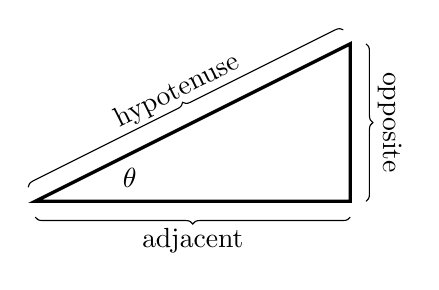
\begin{tikzpicture}
      \coordinate (C) at (0,2);
      \coordinate (D) at (4,2);
      \coordinate (E) at (4,4);
      \tkzMarkRightAngle(C,D,E)
      \tkzMarkAngle(D,C,E)
      \draw[decoration={brace,mirror,raise=.2cm},decorate,thin] (0,2)--(4,2);
      \draw[decoration={brace,mirror,raise=.2cm},decorate,thin] (4,2)--(4,4);
      \draw[decoration={brace,raise=.2cm},decorate,thin] (0,2)--(4,4);
      \draw[very thick] (D)--(E)--(C)--cycle;
      \node at (2,2-.5) {adjacent};
      \node[rotate=-90] at (4+.5,3) {opposite};
      \node[rotate=26.5] at (2-.2,3+.4) {hypotenuse};
      \node at (1.2,2.3) {$\theta$};
    \end{tikzpicture}
  \end{image}
  \vfill
\end{frame}

\begin{frame}
  \vs
  \begin{definition}
    The trigonometric functions are:
    \[
      \begin{aligned}
        \cos(\theta) &= \frac{\text{adj}}{\text{hyp}}\\
        \sec(\theta) &= \frac{1}{\cos(\theta)}
      \end{aligned}
      \qquad
      \begin{aligned}
        \sin(\theta) &= \frac{\text{opp}}{\text{hyp}}\\
        \csc(\theta) &= \frac{1}{\sin(\theta)}
      \end{aligned}
      \qquad
      \begin{aligned}
        \tan(\theta) &= \frac{\sin(\theta)}{\cos(\theta)} \\
        \cot(\theta) &= \frac{\cos(\theta)}{\sin(\theta)}
      \end{aligned}
    \]
    where the domain of sine and cosine is all real numbers, and the
    other are defined precisely when their
    denominators are nonzero.
  \end{definition}
\end{frame}

\begin{frame}
  \vs
  \textbf{The unit circle and trig functions}
  \begin{image}[2.2in]
    \begin{tikzpicture}
      \begin{axis}[
        xmin=-1.1,xmax=1.1,ymin=-1.1,ymax=1.1,
        axis lines=center,
        width=4in,
        xtick={-1,1},
        ytick={-1,1},
        clip=false,
        unit vector ratio*=1 1 1,
        xlabel=$x$, ylabel=$y$,
        every axis y label/.style={at=(current axis.above origin),anchor=south},
        every axis x label/.style={at=(current axis.right of origin),anchor=west},
        ]
        \addplot [dashed, smooth, domain=(0:360)] ({cos(x)},{sin(x)}); %% unit circle

        \addplot [textColor] plot coordinates {(0,0) (.766,.643)}; %% 40 degrees

        \addplot [ultra thick,penColor] plot coordinates {(.766,0) (.766,.643)}; %% 40 degrees
        \addplot [ultra thick,penColor2] plot coordinates {(0,0) (.766,0)}; %% 40 degrees

        % \addplot [ultra thick,penColor3] plot coordinates {(1,0) (1,.839)}; %% 40 degrees

        \addplot [textColor,smooth, domain=(0:40)] ({.15*cos(x)},{.15*sin(x)});
        % \addplot [very thick,penColor] plot coordinates {(0,0) (.766,.643)}; %% sector
        % \addplot [very thick,penColor] plot coordinates {(0,0) (1,0)}; %% sector
        % \addplot [very thick, penColor, smooth, domain=(0:40)] ({cos(x)},{sin(x)}); %% sector
        \node at (axis cs:.15,.07) [anchor=west] {$\theta$};
        \node[penColor, rotate=-90] at (axis cs:.84,.322) {$\sin(\theta)$};
        \node[penColor2] at (axis cs:.383,0) [anchor=north] {$\cos(\theta)$};
        % \node[penColor3, rotate=-90] at (axis cs:1.06,.322) {$\tan(\theta)$};
      \end{axis}
    \end{tikzpicture}
  \end{image}
\end{frame}


\begin{frame}
  \vs
  \textbf{Cosine and its inverse.}
  \begin{image}
    \begin{tikzpicture}
      \begin{axis}[
        xmin=-6.75,xmax=6.75,ymin=-1.5,ymax=1.5,
        axis lines=center,
        xtick={-6.28, -4.71, -3.14, -1.57, 0, 1.57, 3.142, 4.71, 6.28},
        xticklabels={$-2\pi$,$-3\pi/2$,$-\pi$, $-\pi/2$, $0$, $\pi/2$, $\pi$, $3\pi/2$, $2\pi$},
        ytick={-1,1},
        % ticks=none,
        width=6in,
        height=3in,
        unit vector ratio*=1 1.5 1,
        xlabel=$\theta$, ylabel=$x$,
        every axis y label/.style={at=(current axis.above origin),anchor=south},
        every axis x label/.style={at=(current axis.right of origin),anchor=west},
        ]
        \addplot [very thick, penColor2!20!background, samples=100,smooth, domain=(-6.75:0)] {cos(deg(x))};
        \addplot [very thick, penColor2!20!background, samples=100,smooth, domain=(3.14:6.75)] {cos(deg(x))};
        \addplot [very thick, penColor2, samples=100,smooth, domain=(0:3.14)] {cos(deg(x))};

        \addplot[color=penColor2,fill=penColor2,only marks,mark=*] coordinates{(0,1)};  %% closed hole
        \addplot[color=penColor2,fill=penColor2,only marks,mark=*] coordinates{(pi,-1)};  %% closed hole
        \node at (axis cs:-1.57,.75) [penColor2] {$\cos(\theta)$};
      \end{axis}
    \end{tikzpicture}
    %% \caption{The function $\cos(\theta)$ takes on all values between $-1$
    %% and $1$ exactly once on the interval $[0,\pi]$. If we restrict
    %% $\cos(\theta)$ to this interval, then this restricted function has
    %% an inverse.}
    %% \label{figure:cos-restricted}
    %% \end{figure*}
  \end{image}

  \begin{image}[2in]\index{arccosine}
    \begin{tikzpicture}
      \begin{axis}[
        xmin=-1.5,xmax=1.5,ymin=-.25,ymax=3.25,
        axis lines=center,
        ytick={0, 1.57,3.14},
        yticklabels={$0$, $\pi/2$,$\pi$},
        xtick={-1,1},
        unit vector ratio*=1.5 1 1,
        xlabel=$x$, ylabel=$\theta$,
        every axis y label/.style={at=(current axis.above origin),anchor=south},
        every axis x label/.style={at=(current axis.right of origin),anchor=west},
        ]
        \addplot [very thick, penColor5, samples=100,smooth, domain=(-1:1)] {acos(x)*pi/180};
        \addplot[color=penColor5,fill=penColor5,only marks,mark=*] coordinates{(1,0)};  %% closed hole
        \addplot[color=penColor5,fill=penColor5,only marks,mark=*] coordinates{(-1,pi)};  %% closed hole
      \end{axis}
      \node at (3,-1) [text width=2.75in] {Here we see a plot of $\arccos(x)$, the inverse function of
        $\cos(\theta)$ when the domain is restricted to the interval $[0,\pi]$.};
    \end{tikzpicture}
  \end{image}
\end{frame}

\begin{frame}
  \vs
  \textbf{Sine and its inverse.}
  \begin{image}
    \begin{tikzpicture}
      \begin{axis}[
        xmin=-6.75,xmax=6.75,ymin=-1.5,ymax=1.5,
        axis lines=center,
        xtick={-6.28, -4.71, -3.14, -1.57, 0, 1.57, 3.142, 4.71, 6.28},
        xticklabels={$-2\pi$,$-3\pi/2$,$-\pi$, $-\pi/2$, $0$, $\pi/2$, $\pi$, $3\pi/2$, $2\pi$},
        ytick={-1,1},
        % ticks=none,
        width=6in,
        height=3in,
        unit vector ratio*=1 1.5 1,
        xlabel=$\theta$, ylabel=$x$,
        every axis y label/.style={at=(current axis.above origin),anchor=south},
        every axis x label/.style={at=(current axis.right of origin),anchor=west},
        ]
        \addplot [very thick, penColor!20!background, samples=100,smooth, domain=(-6.75:-1.57)] {sin(deg(x))};
        \addplot [very thick, penColor!20!background, samples=100,smooth, domain=(1.57:6.75)] {sin(deg(x))};
        \addplot [very thick, penColor, samples=100,smooth, domain=(-1.57:1.57)] {sin(deg(x))};

        \addplot[color=penColor,fill=penColor,only marks,mark=*] coordinates{(-1.57,-1)};  %% closed hole
        \addplot[color=penColor,fill=penColor,only marks,mark=*] coordinates{(1.57,1)};  %% closed hole
        \node at (axis cs:3.14,.75) [penColor] {$\sin(\theta)$};
      \end{axis}
    \end{tikzpicture}
    %% \caption{The function $\sin(\theta)$ takes on all values between $-1$
    %% and $1$ exactly once on the interval $[-\pi/2,\pi/2]$. If we
    %% restrict $\sin(\theta)$ to this interval, then this restricted
    %% function has an inverse.}
    %% \label{figure:sin-restricted}
    %% \end{figure*}
  \end{image}

  \begin{image}[2in]\index{arcsine}
    \begin{tikzpicture}
      \begin{axis}[
        xmin=-1.5,xmax=1.5,ymin=-1.75,ymax=1.75,
        axis lines=center,
        ytick={-1.57, 0, 1.57},
        yticklabels={$-\pi/2$, $0$, $\pi/2$},
        xtick={-1,1},
        unit vector ratio*=1.5 1 1,
        xlabel=$x$, ylabel=$\theta$,
        every axis y label/.style={at=(current axis.above origin),anchor=south},
        every axis x label/.style={at=(current axis.right of origin),anchor=west},
        ]
        \addplot [very thick, penColor4, samples=100,smooth, domain=(-1:1)] {asin(x)*pi/180};

        \addplot[color=penColor4,fill=penColor4,only marks,mark=*] coordinates{(-1,-pi/2)};  %% closed hole
        \addplot[color=penColor4,fill=penColor4,only marks,mark=*] coordinates{(1,pi/2)};  %% closed hole
      \end{axis}
      \node at (3,-1) [text width=2.75in] {Here we see a plot of $\arcsin(x)$, the inverse function of
        $\sin(\theta)$ when the domain is restricted to the interval $[-\pi/2,\pi/2]$.};
    \end{tikzpicture}
  \end{image}
\end{frame}

\begin{frame}
  \vs
  \textbf{Tangent and its inverse.}
  \begin{image}
    \begin{tikzpicture}
      \begin{axis}[
        xmin=-6.75,xmax=6.75,ymin=-3,ymax=3,
        axis lines=center,
        width=6in,
        height=3in,
        xtick={-6.28, -4.71, -3.14, -1.57, 0, 1.57, 3.142, 4.71, 6.28},
        xticklabels={$-2\pi$,$-3\pi/2$,$-\pi$, $-\pi/2$, $0$, $\pi/2$, $\pi$, $3\pi/2$, $2\pi$},
        unit vector ratio*=1 1 1,
        xlabel=$\theta$, ylabel=$x$,
        every axis y label/.style={at=(current axis.above origin),anchor=south},
        every axis x label/.style={at=(current axis.right of origin),anchor=west},
        ]
        \addplot [very thick, penColor3, samples=100,smooth, domain=(-1.55:1.55)] {tan(deg(x))};
        \addplot [very thick, penColor3!30!background, samples=100,smooth, domain=(-4.69:-1.59)] {tan(deg(x))};
        \addplot [very thick, penColor3!30!background, samples=100,smooth, domain=(-6.75:-4.73)] {tan(deg(x))};
        \addplot [very thick, penColor3!30!background, samples=100,smooth, domain=(1.59:4.69)] {tan(deg(x))};
        \addplot [very thick, penColor3!30!background, samples=100,smooth, domain=(4.73:6.75)] {tan(deg(x))};

        \addplot [textColor,dashed] plot coordinates {(-4.71,-3) (-4.71,3)};
        \addplot [textColor,dashed] plot coordinates {(-1.57,-3) (-1.57,3)};
        \addplot [textColor,dashed] plot coordinates {(1.57,-3) (1.57,3)};
        \addplot [textColor,dashed] plot coordinates {(4.71,-3) (4.71,3)};

        \node at (axis cs:.4,1.25) [penColor3] {$\tan(\theta)$};
      \end{axis}
    \end{tikzpicture}
    %% \caption{The function $\tan(\theta)$ takes on all values in $\R$
    %% exactly once on the open interval $(-\pi/2,\pi/2)$. If we restrict
    %% $\tan(\theta)$ to this interval, then this restricted function has
    %% an inverse.}
    %% \end{figure*}
    %% \end{fullwidth}
  \end{image}

  \begin{image}
    \begin{tikzpicture}
      \begin{axis}[
        xmin=-6,xmax=6,ymin=-2,ymax=2,
        axis lines=center,
        ytick={0, -1.57,1.57},
        width=6in,
        height=3in,
        yticklabels={$0$, $-\pi/2$,$\pi/2$},
        xtick={0},
        unit vector ratio*=1 1 1,
        xlabel=$x$, ylabel=$\theta$,
        every axis y label/.style={at=(current axis.above origin),anchor=south},
        every axis x label/.style={at=(current axis.right of origin),anchor=west},
        ]
        \addplot [very thick, penColor3!20!penColor2, samples=100,smooth, domain=(-6:6)] {atan(x)*pi/180};
        \addplot [textColor,dashed] plot coordinates {(-6,-1.57) (6,-1.57)};
        \addplot [textColor,dashed] plot coordinates {(-6,1.57) (6,1.57)};
      \end{axis}
      \node at (7,-1) [text width=5in] {Here we see a plot of $\arctan(x)$, the inverse function of
        $\tan(\theta)$ when the domain is restricted to the interval $(-\pi/2,\pi/2)$.};
    \end{tikzpicture}
    %% \caption{Here we see a plot of $\arctan(y)$, the inverse function of
    %% $\tan(\theta)$ when it is restricted to the interval $(-\pi/2,\pi/2)$.}
    %% \end{figure*}
    %% \index{arctangent}
    %% \end{fullwidth}
  \end{image}
\end{frame}

\begin{frame}
  \vs
  \textbf{Pythagorean theorem and identities.}
  \begin{image}[0.5\textwidth]
    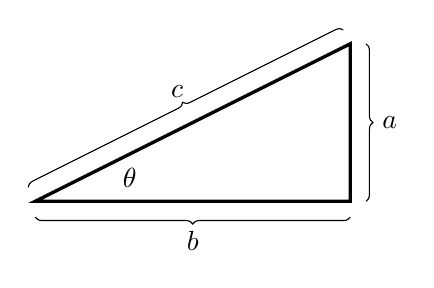
\begin{tikzpicture}
      \coordinate (C) at (0,2);
      \coordinate (D) at (4,2);
      \coordinate (E) at (4,4);
      \tkzMarkRightAngle(C,D,E)
      \tkzMarkAngle(D,C,E)
      \draw[decoration={brace,mirror,raise=.2cm},decorate,thin] (0,2)--(4,2);
      \draw[decoration={brace,mirror,raise=.2cm},decorate,thin] (4,2)--(4,4);
      \draw[decoration={brace,raise=.2cm},decorate,thin] (0,2)--(4,4);
      \draw[very thick] (D)--(E)--(C)--cycle;
      \node at (2,2-.5) {$b$};
      \node[] at (4+.5,3) {$a$};
      \node at (2-.2,3+.4) {$c$};
      \node at (1.2,2.3) {$\theta$};
    \end{tikzpicture}
  \end{image}
  \hfill
  \begin{minipage}[t]{0.45\textwidth}
    Pythagorean theorem:
    \begin{itemize}
    \item $a^2 + b^2 = c^2$
    \end{itemize}
  \end{minipage}
  \begin{minipage}[t]{0.45\textwidth}
    Pythagorean identities:
    \begin{itemize}
    \item $\cos^2\theta+\sin^2\theta = 1$
    \item $1 + \tan^2\theta = \sec^2\theta$
    \item $\cot^2\theta + 1 = \csc^2\theta$
    \end{itemize}
  \end{minipage}
  \hfill
\end{frame}


\begin{frame}
  \frametitle{Exponential and logarithmic functions}
  \begin{definition}
    An \dfn{exponential function} is a function of the form
    \[
      f(x) = b^x
    \]
    where  $b\ne 1$ is a positive real number. The domain of an
    exponential function is $(-\infty,\infty)$. (Special: $f(x) = e^x$.)
  \end{definition}

  \begin{image}[0.4\textwidth]
    \begin{tikzpicture}
      \begin{axis}[
        domain=-2:2,
        xmin=-2, xmax=2,
        ymin=-.5, ymax=4,
        axis lines =middle, xlabel=$x$, ylabel=$y$,
        every axis y label/.style={at=(current axis.above origin),anchor=south},
        every axis x label/.style={at=(current axis.right of origin),anchor=west},
        ]
	\addplot [very thick, penColor, smooth] {2^x};
        \addplot [very thick, penColor2, smooth] {2^(-x)};
        \node at (axis cs:-2.1, 2 ) [penColor2,anchor=west] {$0 < b < 1$};
        \node at (axis cs:1.2, 2 ) [penColor,anchor=west] {$b > 1$};
      \end{axis}
    \end{tikzpicture}
  \end{image}
\end{frame}

\begin{frame}
  \vs
  \begin{definition}
    A \dfn{logarithmic function} is a function defined as follows
    \[
      \log_b(x) = y \qquad\text{means that}\qquad b^y = x
    \]
    where  $b\ne 1$ is a positive real number. The domain of a
    logarithmic function is $(0,\infty)$. (Special: $f(x) = \ln (x)$.)
  \end{definition}
  \begin{image}[0.45\textwidth]
    \begin{tikzpicture}
      \begin{axis}[
        domain=0.05:4,
        xmin=-.5, xmax=4,
        ymin=-2, ymax=2,
        axis lines =middle, xlabel=$x$, ylabel=$y$,
        every axis y label/.style={at=(current axis.above origin),anchor=south},
        every axis x label/.style={at=(current axis.right of origin),anchor=west},
        ]
        \addplot [very thick, penColor2, smooth, samples=100]
        {ln(x)/ln(1/2))}; % 0 < b < 1
        \addplot [very thick, penColor, smooth] {ln(x)/ln(2)}; % b > 1

        \node at (axis cs:.5, 1.3 ) [penColor2,anchor=west] {$0 < b < 1$};
        \node at (axis cs:.5, -1.3 ) [penColor,anchor=west] {$b > 1$};
      \end{axis}
    \end{tikzpicture}
  \end{image}
\end{frame}

\begin{frame}
  \vs
  \begin{block}{Properties of exponents}
    Let $b$ be a positive real number with $b\ne 1$.
    \begin{itemize}
    \item $\ds b^m\cdot b^n = b^{m+n}$
    \item $\ds b^{-1} = \frac{1}{b}$
    \item $\ds \left(b^m\right)^n = b^{mn}$
    \end{itemize}
  \end{block}
  \vfill
  \begin{block}{Properties of logarithms}
    Let $b$ be a positive real number with $b\ne 1$.
    \begin{itemize}
    \item $\ds \log_b(m\cdot n) = \log_b(m) + \log_b(n)$
    \item $\ds \log_b(m^n) = n\cdot \log_b(m)$
    \item $\ds \log_b\left(1/m\right) = \log_b(m^{-1}) = -\log_b(m)$
    \item $\ds \log_a(m) = \frac{\log_b(m)}{\log_b(a)}$
    \end{itemize}
  \end{block}
  \vfill
\end{frame}

\end{document}


%%% Local Variables:
%%% mode: latex
%%% TeX-master: t
%%% End:
